% Created 2023-05-06 Sat 18:40
% Intended LaTeX compiler: pdflatex
\documentclass[14pt]{extarticle}
\usepackage[utf8]{inputenc}
\usepackage[T1]{fontenc}
\usepackage{graphicx}
\usepackage{longtable}
\usepackage{wrapfig}
\usepackage{rotating}
\usepackage[normalem]{ulem}
\usepackage{amsmath}
\usepackage{amssymb}
\usepackage{capt-of}
\usepackage{hyperref}
\usepackage[a4paper]{geometry}
\usepackage[T2A]{fontenc}
\usepackage[utf8]{inputenc}
\usepackage[ukrainian, ]{babel}
\usepackage{enumitem}
\usepackage{amsmath}
\usepackage{hyperref}
\usepackage{titlesec}
\usepackage{tikz}
\usepackage{pgfplots}
\usetikzlibrary{positioning}
\usetikzlibrary{shapes.geometric}
\usepackage{lastpage}
\usepackage{graphicx}
\graphicspath{ {./report/images/} }

\usepackage[backend=biber]{biblatex}
\addbibresource{references.bib}

\renewcommand{\baselinestretch}{1.2}

\author{Кирило Байбула, ДО-3}
\date{\today}
\title{Курсова робота на тему: Аналіз на ПК СМО M/G/n/m}
\hypersetup{
 pdfauthor={Кирило Байбула, ДО-3},
 pdftitle={Курсова робота на тему: Аналіз на ПК СМО M/G/n/m},
 pdfkeywords={},
 pdfsubject={Аналіз на ПК СМО M/G/n/m},
 pdfcreator={Emacs 28.2 (Org mode 9.6.1)}, 
 pdflang={Ua}}

\begin{document}

% \fontsize{14pt}{16pt}\selectfont

\begin{titlepage}
\begin{center}
\textbf{КИЇВСЬКИЙ НАЦІОНАЛЬНИЙ УНІВЕРСИТЕТ ІМЕНІ ТАРАСА ШЕВЧЕНКА} \\
Факультет комп'ютерних наук та кібернетики \\
Кафедра дослідження операцій \\
\vspace{2cm}
{\Large \textbf{КУРСОВА РОБОТА} \par}
на тему: \\
\textbf{Аналіз на ПК СМО M/G/n/m} \\
\vspace{2cm}
{\large }
\end{center}
\begin{flushright}
\vfill
студента 3 курсу \\
Байбула Кирило Аленовича
\vfill
Науковий керівник: \\
професор, доктор фізико-математичних наук \\
Мацак Іван Каленикович
\end{flushright}
\vfill
\begin{center}
Київ --- 2023
\end{center}
\end{titlepage}

\section*{Реферат}

Обсяг роботи \pageref{LastPage} сторінок.

ДОСЛІДЖЕННЯ СИСТЕМ МАСОВОГО ОБСЛУГОВУВАННЯ ІЗ ОБМЕЖЕНОЮ ЧЕРГОЮ M/G/n/m.

Об\textquoterightєктом дослідження є система масового обслуговування з обмеженою чергою
\(M/G/n/m\). Предметом роботи є розробка імітаційної моделі системи масового
обслуговування з обмеженою чергою та аналіз результатів її роботи.

Метою роботи є знаходження загальних характеристик подібної системи, таких як:
середній час очікування та середня довжина черги. Також досліджується вплив
зміни параметрів системи на її продуктивність. Зокрема, аналіз того, як
швидкість прибуття, швидкість обслуговування та місткість черги впливають на
продуктивність системи.

Методи розроблення: комп\textquotesingleютерне моделювання. Інструменти
розроблення: мова програмування Rust та вільно поширюване інтегроване середовище
розробки Emacs 28.2.

\newpage

\setcounter{tocdepth}{2}
\tableofcontents
\newpage

\section{Перелік умовних позначень, символів, скорочень}
\begin{table}[h!]
  \centering
  \begin{tabular}{ c c l }
    СМО &:& система масового обслуговування. \\
    \(\Theta(t)\) &:& довжина черги (стан) СМО в момент часу \(t\); \\
    \(P_{k}\) &:& стаціонарна ймовірність того, що в системі є \(k\) запитів; \\
    \(W_{i}\) &:& час очікування \(i\)-ого запиту у черзі; \\
  \end{tabular}
\end{table}

\newpage

\section{Вступ}\label{sec:intro}

Курсова робота присвячена дослідженню систем масового обслуговування із
обмеженою чергою. Подібні системи використовуються для моделювання різноманітних
процесів, де можуть виникати черги, наприклад, у телекомунікаційних мережах,
медичних установах, аеропортах, ресторанах, тощо.

Подібні системи ми будемо називати СМО із обмеженою чергою \(M/G/n/m\), якщо:

\begin{enumerate}
  \item Запити до СМО надходять як \textbf{М}акрківський (Пуассонівський)
        процес, що має параметр \(\lambda > 0\) (тобто \(\tau_{i+1} = t_{i+1} - t_{i}\) ---
        час між надходженнями \(i\)-ого та \(i+1\) запиту має експоненційний
        розподіл з параметром \(\lambda\));
  \item Час обробки кожного запиту СМО визначен випадковою величиною \(\xi\), що
        має довільний розподіл \(G(x)\).
  \item СМО має \(n\) приладів, що обробляють запити із черги;
  \item СМО має чергу з довжиною не більше ніж \(m\) (тобто система не може
        тримати більше ніж \(m\) запитів у черзі, а максимальна кількість
        запитів, що може бути прийнята системою, дорівнює сумі кількості
        приладів і максимальної довжини черги, тобто --- \(n + m\));
\end{enumerate}

Кожен новий запит, що надходить у систему, спочатку призначається для будь-якого незайнятого приладу обслуговування. Інакше, якщо всі прилади зайняті, запит стає у чергу для подальшого оброблення.

\begin{figure}
\begin{tikzpicture}[
roundnode/.style={circle, draw=black!60, fill=black!5, very thick, minimum size=7mm},
squarednode/.style={rectangle, draw=black!60, fill=black!5, very thick, minimum size=5mm},
rombnode/.style={diamond, draw=black!60, fill=black!5, very thick, minimum size=5mm},
]

% Add  some colored background to highlight requests queue
\fill[gray!20] (1,-1) rectangle (10.5,1);
\node[draw] at (2.7,-1.4) {Черга запитів};

% Arrival nodes
\node[rombnode]      (markovianarrival)                           {\(\lambda\)};

% Queue nodes
\node[roundnode]        (requesti)          [right=of markovianarrival] {\(r_{i}\)};
\node[roundnode]        (requestother)          [right=of requesti]         {\ldots};
\node[roundnode]        (request3)          [right=of requestother]         {\(r_{3}\)};
\node[roundnode]        (request2)      [right=of request3]        {\(r_{2}\)};
\node[roundnode]        (request1)          [right=of request2]     {\(r_{1}\)};

% Service nodes
\node[squarednode]      (service3)       [right=of request1]         {\(S_{3}\)};
\node[squarednode]      (service2)       [above=of service3]         {\(S_{2}\)};
\node[squarednode]      (service1)       [above=of service2]         {\(S_{1}\)};
\node[squarednode]      (serviceother)   [below=of service3]         {\ldots};
\node[squarednode]      (servicen)       [below=of serviceother]     {\(S_{n}\)};

% Departure node
\node[rombnode]        (departure)      [right=of service3]         {\(G(x)\)};

\draw[->] (markovianarrival) -- (requesti);
\draw[->] (requesti) -- (requestother);
\draw[->] (requestother) -- (request3);
\draw[->] (request3) -- (request2);
\draw[->] (request2) -- (request1);
\draw[->] (request1) -- (service1);
\draw[->] (request1) -- (service2);
\draw[->] (request1) -- (service3);
\draw[->] (request1) -- (serviceother);
\draw[->] (request1) -- (servicen);
\draw[->] (service1) -- (departure);
\draw[->] (service2) -- (departure);
\draw[->] (service3) -- (departure);
\draw[->] (serviceother) -- (departure);
\draw[->] (servicen) -- (departure);
\end{tikzpicture}
\caption{Схема роботи \(M/G/n/m\), де \(r_{i}\) --- \(i\)-тий запит у черзі,
  \(S_{n}\) --- \(n\)-тий прилад. }\label{fig:mgnm}
\end{figure}

Головною метою данної роботи є знаходження стаціонарних характеристик СМО, таких
як:

\begin{enumerate}
  \item \(P_{k} = P\{\Theta = k\} = \lim_{t \to \infty}P\{\Theta(t) = k\}, k = 0,1,2 \ldots n+m\);
  \item \(\mathbb{M} \Theta_k = \lim_{t \to \infty} \mathbb{M} \Theta(t)\);
  \item \(\mathbb{M} W = \lim_{k \to \infty} W_k \);
\end{enumerate}

Тобто, ми хочемо знайти стаціонарний розподіл кількості запитів у системі, середню
кількість запитів у системі та середній час очікування запиту у черзі.

Через складність дослідження та аналізу подібної СМО, ми будемо використовувати
метод Монте-Карло, тобто змоделєюмо та запрограмуємо систему за допомогою
комп'ютера та зробимо велику кількість експериментів, що дозволить нам знайти та
проаналізувати бажані характеристики.

\newpage

\section{Теоретичні відомості}

У цьому розділі будуть предоставлені короткі теоретичні відомості про системи
масового обслуговування з переглядом їх основних видів, що надасть нам
фундамент для дослідження та аналізу нашої СМО.

\subsection{СМО типу \(M/M/c/K\)}\label{sec:mmck}

Цікавим для огляду буде система масового обслуговування \(M/M/c/K\), що має так
само на вхід Марківський потік запитів та обмежену кількість приладів
обслуговування кількістю \(c\) та скінчену чергу максимальною довжиною \(K\),
але, на відмінну від \(M/G/n/m\), має експоненціальний час обслуговування із
параметром \(\mu\). Тобто, \(M/M/c/K\) --- це частковий випадок \(M/G/n/m\).

\begin{figure}[h!]
\begin{tikzpicture}[
roundnode/.style={circle, draw=black!60, fill=black!5, very thick, minimum size=7mm},
squarednode/.style={rectangle, draw=black!60, fill=black!5, very thick, minimum size=5mm},
rombnode/.style={diamond, draw=black!60, fill=black!5, very thick, minimum size=5mm},
]

% Add  some colored background to highlight requests queue
\fill[gray!20] (1,-1) rectangle (10.5,1);
\node[draw] at (5.7,-1.4) {Черга запитів макс. довжиною \(K\)};

% Arrival nodes
\node[rombnode]      (markovianarrival)                           {\(\lambda\)};

% Queue nodes
\node[roundnode]        (requesti)          [right=of markovianarrival] {\(r_{i}\)};
\node[roundnode]        (requestother)          [right=of requesti]         {\ldots};
\node[roundnode]        (request3)          [right=of requestother]         {\(r_{3}\)};
\node[roundnode]        (request2)      [right=of request3]        {\(r_{2}\)};
\node[roundnode]        (request1)          [right=of request2]     {\(r_{1}\)};

% Service nodes
\node[squarednode]      (service3)       [right=of request1]         {\(S_{3}\)};
\node[squarednode]      (service2)       [above=of service3]         {\(S_{2}\)};
\node[squarednode]      (service1)       [above=of service2]         {\(S_{1}\)};
\node[squarednode]      (serviceother)   [below=of service3]         {\ldots};
\node[squarednode]      (servicen)       [below=of serviceother]     {\(S_{c}\)};

% Departure node
\node[rombnode]        (departure)      [right=of service3]         {\(\lambda\)};

\draw[->] (markovianarrival) -- (requesti);
\draw[->] (requesti) -- (requestother);
\draw[->] (requestother) -- (request3);
\draw[->] (request3) -- (request2);
\draw[->] (request2) -- (request1);
\draw[->] (request1) -- (service1);
\draw[->] (request1) -- (service2);
\draw[->] (request1) -- (service3);
\draw[->] (request1) -- (serviceother);
\draw[->] (request1) -- (servicen);
\draw[->] (service1) -- (departure);
\draw[->] (service2) -- (departure);
\draw[->] (service3) -- (departure);
\draw[->] (serviceother) -- (departure);
\draw[->] (servicen) -- (departure);
\end{tikzpicture}
\caption{Схема роботи \(M/G/c/K\), де \(r_{i}\) --- \(i\)-тий запит у черзі,
  \(S_{c}\) --- \(c\)-тий прилад. }\label{fig:mmck}
\end{figure}

Ця модель може бути представлена у вигляді ланцюга Марківських станів, із
матрицею переходів:

\begin{equation*}
  Q = \begin{pmatrix}
       -\lambda & \lambda  \\
        \mu & -(\lambda + \mu) & \lambda \\
          & 2\mu & -(\lambda + 2\mu) & \lambda \\
          & & \ddots & \ddots & \ddots \\
          & & & c\mu & -(\lambda + c\mu) & \lambda \\
          & & & & \ddots & \ddots & \ddots \\
          & & & & & c \mu & -c\mu \\
  \end{pmatrix}
\end{equation*}

на просторі станів \(\{0,1,2,\ldots,K\}\). Подібний ланцюг називають процесом ``смерті-народження'' (birth-death process), де переходи бувають лише двох видів:
\textit{народження}, що збільшує змінну стану на одиницю, та \textit{смерть},
що зменшує її на одиницю \cite{willy-feller}. Саме тому, простіше представити
матрицю переходів у вигляді машини станів:

\begin{figure}[h!]
  \centering
  \begin{tikzpicture}[
    roundnode/.style={circle, draw=black!60, fill=black!5, very thick, minimum size=7mm},
  ]
  \node[roundnode]        (state0)          {\(0\)};
  \node[roundnode]        (state1)       [right=of state0]        {\(1\)};
  \node[roundnode]        (state2)       [right=of state1]        {\(2\)};
  \node[roundnode]        (stateother)   [right=of state2]        {\(\cdots\)};
  \node[roundnode]        (statec)       [right=of stateother]        {\(c\)};
  \node[roundnode]        (stateotherc)   [right=of statec]        {\(\cdots\)};
  \node[roundnode]        (stateK)       [right=of stateotherc]        {\(K\)};

  \draw[->] (state0) edge[bend left=20] node[above] {\(\lambda\)} (state1);
  \draw[->] (state1) edge[bend left=20] node[below] {\(\mu\)} (state0);
  \draw[->] (state1) edge[bend left=20] node[above] {\(\lambda\)} (state2);
  \draw[->] (state2) edge[bend left=20] node[below] {\(\mu\)} (state1);
  \draw[->] (state2) edge[bend left=20] node[above] {\(\lambda\)} (stateother);
  \draw[->] (stateother) edge[bend left=20] node[below] {\(\mu\)} (state2);
  \draw[->] (stateother) edge[bend left=20] node[above] {\(\lambda\)} (statec);
  \draw[->] (statec) edge[bend left=20] node[below] {\(\mu\)} (stateother);
  \draw[->] (statec) edge[bend left=20] node[above] {\(\lambda\)} (stateotherc);
  \draw[->] (stateotherc) edge[bend left=20] node[below] {\(\mu\)} (statec);
  \draw[->] (stateotherc) edge[bend left=20] node[above] {\(\lambda\)} (stateK);
  \draw[->] (stateK) edge[bend left=20] node[below] {\(\mu\)} (stateotherc);
\end{tikzpicture}
\caption{Машина станів \(M/M/c/K\)}\label{fig:mmck-fsm}
\end{figure}

Також важливою характеристою СМО, є \textbf{утілизація}. Утілизація --- це
відношення часу, коли пристрій зайнятий, до загального часу. Для \(M/M/c/K\)
утілизація має вигляд:

\begin{equation}
  \rho = \frac{\lambda}{c\mu}
\end{equation}\label{eq:mmck-utilization}

При цьому ж, \(\rho\) має обмеження \(\rho < 1\), що відповідає тому, що система
не може обслуговувати запити швидше, ніж вони надходять. Інакше, система
буде постійно переповнбювати чергу і губити запити.

Стаціонарний розподіл кількості запитів у системі \(P_{k}\) для \(M/M/c/K\) був
наведений ще у 1981 році \cite{allen} та має вигляд:

\begin{equation}
\begin{aligned}
  P_{0} & = \left[ \sum_{k=0}^{c} \frac{\lambda^{k}}{\mu^{k}k!} + \frac{\lambda^{c}}{\mu^{c} c!} \sum_{k = c+1}^{K} \frac{\lambda^{k-c}}{\mu^{k-c}c^{k-c}} \right]^{-1} \\
  P_{k} & = \left\{
      \begin{aligned}
        &\frac{\lambda^{k}}{\mu^{k}k!}P_{0}, & k = 1,2,\ldots,c \\
        &\frac{\lambda^{k}}{\mu^{k}c^{k-c}c!}P_{0}, & k = c+1,c+2,\ldots,K
      \end{aligned}
  \right.
\end{aligned}
\end{equation}\label{eq:mmck-sp}

Середня кількість часу проведеного запитом у системі:

\begin{equation}
  W = \frac{1}{\mu} + P_{0} \frac{\rho{(c \rho)}^{c}}{\lambda{(1-\rho)}^{2}c!}
\end{equation}\label{eq:mmck-wm}

Середня кількість часу очікування запиту у черзі:

\begin{equation}
  W_{q} = P_{0} \frac{\rho{(c \rho)}^{c}}{\lambda{(1-\rho)}^{2}c!}
\end{equation}\label{eq:mmck-wq}

І звідси ж, за формулою Літтла, середня кількість запитів у системі:

\begin{equation}
  \mathbb{M} \Theta = \lambda W = \frac{\lambda}{\mu} + P_{0} \frac{\rho(c \rho)^{c}}{(1-\rho)^{2}c!}
\end{equation}\label{eq:mmck-mql}

\subsection{СМО типу \(M/G/n/m\)}
Як було зазначено вище, СМО типу \(M/G/n/m\) є більш загальним випадком СМО типу
\(M/M/c/K\) (див \ref{sec:mmck}), де \(G\) --- це загальний розподіл часу обслуговування
запиту (також див. \ref{sec:intro}). Саме тому, \(M/G/n/m\) має багато спільних
властивостей з \(M/M/c/K\), але, через невизначеність, загальність \(G\),
\(M/G/n/m\) --- є важким для аналітичного дослідження.

Tijms та ін. вважають, що \textit{"малоймовірно, що можна розробити методи для
  обчислення точних числових значень стаціонарної ймовірності в черзі
  \(M/G/k\)"} \cite{tijms}.

Саме тому, для \(M/G/n/m\) спробуємо використати інший підхід, а саме ---
моделювання.

\newpage

\section{Моделювання СМО}

У даному розділі буде розглянуто підходи до моделювання СМО, що дозволить нам
вибрати найбільш оптимальний підхід для нашої задачі. Починаючи з огляду
архітектури системи, закінчуючи описом алгоритму моделювання.

\subsection{Імітаційна модель}
Одним із підходів, зазначених у \cite{wiley}, є побудова моделі, що буде працювати з
імітованим, дискретним часом, де кожен крок системи є фіксованим інтервалом.
Неперервні розподіли, таким чином, стають дискретними, що призводить до
округлення помилок. І звідси, єдиний спосіб зменшити розмір помилки --- зменьшити
крок часу. З іншого боку, з цього випливає і збільшення часу роботи програмної
моделі.

Саме тому, у \cite{tits-veeken} було запропоновано імітаційну модель, що працює зі зміними
кроками часу, що базуються на подіях, що виникають у самій системі. Тобто кожен
наступний крок --- стрибок у часі від останньої події до найближчої наступної. Тим
самим ми пришвидшуємо роботу імітаціної моделі у декілька разів та позбавляємося
від дискретності у часі.

\subsection{Моделюючий алгоритм}
Параметрами нашої моделі будуть:

\begin{enumerate}
  \item \(n\) --- кількість приладів обслуговування;
  \item \(m\) --- довжина черги;
  \item \(\lambda\) --- інтенсивність надходження запитів;
  \item \(G(x)\) --- розподіл часу обслуговування запитів. На приктиці буде або
        експоненційним (завдяки чому система буде перетворюватися у СМО типу
        \(M/M/c\) \cite{3}), або рівномірним;
  \item \(T\) --- час життя моделі.
\end{enumerate}

Також головними об\textquoteright єктами моделювання є:

\begin{enumerate}
  \item \(t\) --- теперішній час моделі;
  \item \(Q\) --- черга запитів;
  \item \(E\) --- відсортована по часу черга подій. Елементи цією черги бувають
        двох видів: запит, що прибув у систему, та запит, що вийшов з системи;
  \item \(S\) --- множина приладів обслуговування;
  \item \(r_{i}(t)\) --- \(i\)-тий запит, що має параметр \(t\) --- час потрібний
        приладу для обслуговування запитів;
  \item \(Rand_{P}\) --- підпрограма, що генерує випадкові числа з експоненційним
        розподілом, що визначаюють наступний час прибуття запиту;
  \item \(Rand_{G}\) --- підпрограма, що генерує випадкові числа з розподілом
        \(G(x)\), що визначають час обслуговування запиту.
\end{enumerate}

Таким чином, все життя системи буде складатися з послідовного ітерування по
подіям із черги \(E\). Якщо подія --- прибуття запиту, то він додається до черги
\(Q\), і, за допомогою підпрограми \(Rand_{P}\), генерується час наступного
прибуття запиту. що також додається до черги \(E\). Якщо подія --- виходження
запиту, то запит позначається як виконаний, і, якщо черга \(Q\) не пуста, то з
неї видаляється наступний запит, а у чергу \(E\) додається подія виходження
цього запиту, час котрого визначається за допомогою підпрограми \(Rand_{G}\).

Приклад  імплементації можна побачити у репозиторії \cite{Baybula_Analyze_on_PC_2023}.

\newpage

\section{Результати моделювання}

Провівши декілька експериментів на імітаційній моделі із фіксованими
параметрами, можемо розглянути результати.

\subsection{\(G(x)\)  --- екпоненційний розподіл}

Розглянемо випадок, коли \(G(x)\) --- експоненційний розподіл. Фактично, це є
частковим випадком СМО \(M/M/c/K\), що описуна у \ref{sec:mmck}.

Змоделюємо ситуацію з \(n = 5\) приладами обслуговування, довжиною черги
\(m = 30\), очікуваним часом обслуговування \(1 / \lambda = 26\) секунд, з очікуваним
періодом надходження запитів \(1 / \mu = 4\) секунд.

При \(T = 10,000\) секунд, розглянемо кількість запитів в залежності від часу
(рис. \ref{img:exp-fail-first-requests}). Бачимо, що кількість запитів у системі
коливається від 25 до 35 із частими піками саме до 35, що свідчить про втрати,
пов\textquoteright язані з переповненням черги. Що і не дивно, враховуючи
утилізацію \(M/M/c/k\) \ref{eq:mmck-utilization} :

\begin{equation*}
  \rho = \frac{\lambda}{c \mu} = \frac{26}{5 \cdot 4} = 1.3 \ngtr 1
\end{equation*}

Подібну систему не можна вважати ефектичною, саме тому спробуймо зменьшити
очікуваний час обслуговування так, щоб враховувалася умова
\ref{eq:mmck-utilization}.

\begin{figure}
  \centering
  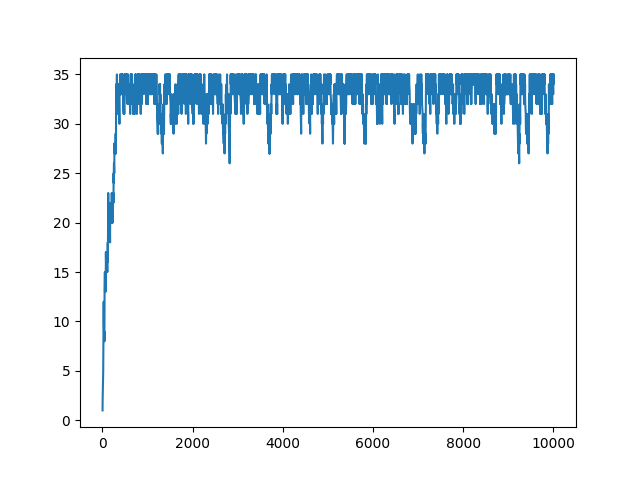
\includegraphics{fail-seconds-requests_in_system.png}\caption{{Залежність
      кількісті запитів від часу при \(1/\lambda = 26\), \(n = 5\),
      \(1/\mu = 4\)}}\label{img:exp-fail-first-requests}
\end{figure}

При \(1 / \lambda = 19\), \(n = 5\), \(1 / \mu = 4\), \(m = 30\), \(T = 10,000\) секунд,
утилізація становитиме: \(\rho = 0.95 > 1\). З рис. \ref{img:exp-first-requests}
бачимо графік станів із піками, що не перевищують максимальну кількість запитів
у системі, тобто система не втрачає запити, а отже є ефективною.

\begin{figure}
  \centering
  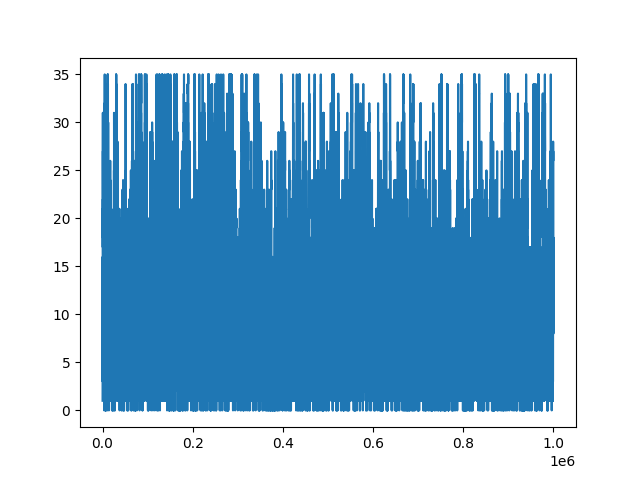
\includegraphics{10_000_seconds-requests_in_system.png}\caption{{Залежність кількісті
      запитів від часу при \(1/\lambda = 19\), \(n = 5\),
      \(1/\mu = 4\)}}\label{img:exp-first-requests}
\end{figure}

Розглянемо також кумулятивну середню кількість запитів у системі (рис.
\ref{img:exp-queue-length-mean-10-000}). Бачимо, невизначені коливання.

Так як, нам потрібно розглянути стаціонарні характеристи при \(t \to \infty\),
спробуємо смоделювати систему при \(T = 1,000,000\) (рис.
\ref{img:exp-first-requests}). Звідси, бачимо, кумулятивне середнє при \(t \to \infty\)
наближається до фіксованого значення \(\approxeq 11.5\).

\begin{figure}
  \centering
  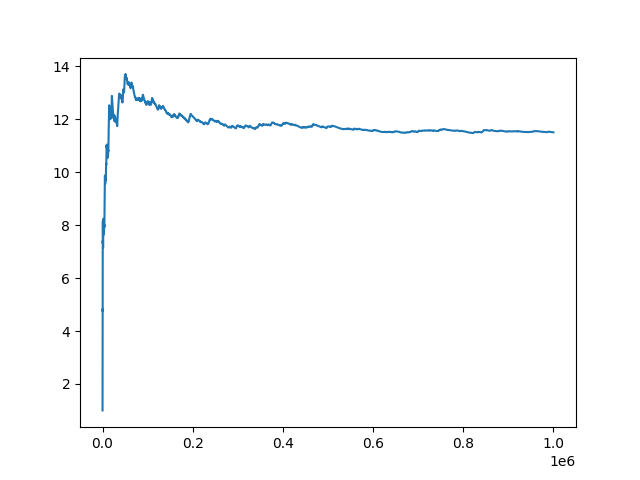
\includegraphics{10_000_seconds-queue_length_mean.png}\caption{{Залежність
      кумулятивної середньої кількості запитів у черзі від часу при
      \(1/\lambda = 19\), \(n = 5\), \(1/\mu = 4\) та
      \(T = 10,000\)}}\label{img:exp-queue-length-mean-10-000}
\end{figure}

\begin{figure}
  \centering
  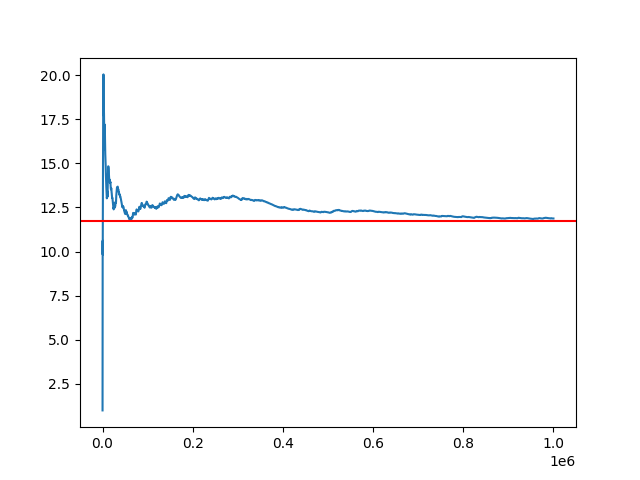
\includegraphics{1_000_000_seconds-queue_length_mean.png}\caption{{Залежність
      кумулятивної середньої кількості запитів у черзі від часу при
      \(1/\lambda = 19\), \(n = 5\), \(1/\mu = 4\) та \(T = 1,000,000\). Червона лінія
      \(y = 11.75\)}}\label{img:exp-queue-length-mean-1-000-000}
\end{figure}

Так само і для середньої кількості часу очікування запиту в черзі (рис. \ref{img:exp-wait-time-mean-1-000-000}).

\begin{figure}
  \centering
  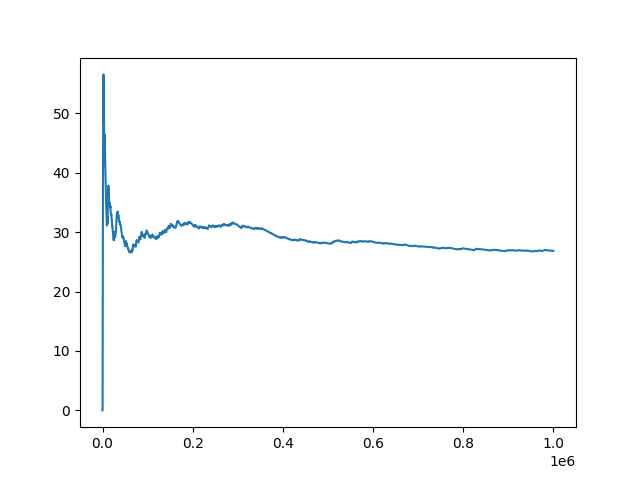
\includegraphics{1_000_000_seconds-waiting_mean.png}\caption{{Залежність
      середньої кількості часу у черзі від часу при \(1/\lambda = 19\), \(n = 5\),
      \(1/\mu = 4\) та
      \(T = 1,000,000\)}}\label{img:exp-wait-time--mean-1-000-000}
\end{figure}

\newpage

\section{Висновки}

Аналізуючи дані експерименту з моделлю \(M/G/n/m\) чергової системи, ми дійшли
до висновку, що через загальну природу СМО, з невизначеним розподілом \(G(x)\), для ефективного аналізу краще використовувати наступний підхід:

\begin{enumerate}
  \item Розглянути можливі випадки
\end{enumerate}

\newpage

\printbibliography

\end{document}
